\documentclass[conference]{IEEEtran}

\usepackage{cite}
\usepackage{amsmath,amssymb,amsfonts}
\usepackage{algorithmic}
\usepackage{graphicx}
\usepackage{textcomp}
\usepackage{xcolor}

\def\BibTeX{{\rm B\kern-.05em{\sc i\kern-.025em b}\kern-.08em
  T\kern-.1667em\lower.7ex\hbox{E}\kern-.125emX}}
\begin{document}

\title{Decentralized Access Control}%*\\

\author{
  \IEEEauthorblockN{
    1\textsuperscript{st} Heinrich Lorenz}
    \IEEEauthorblockA{\textit{dept. name of organization (of Aff.)} \\
    \textit{name of organization (of Aff.)}\\
    Karlsruhe, Germany \\
    lorenz.heinrich@student.kit.edu}
}

\maketitle

\begin{abstract}
  Lorem ipsum dolor sit amet, consectetur adipiscing elit. sed non risus. Suspendisse lectus tortor, dignissim sit amet, adipiscing nec, ultricies sed, dolor. Cras elementum ultrices diam.
\end{abstract}

\begin{IEEEkeywords}
  lorem, ipsum, dolor, sit, amet
\end{IEEEkeywords}

\section{Introduction}
lorem ipsum dolor sit amet, consectetur adipiscing elit. sed non risus.

\section{Access Control}
For users of the modern web, granting service providers access to protected resources is a common practice and is often required to even use certain web services.
A system offering access control essentially enables users to disclose resources owned by them for usage by the requesting web service.
Desired attributes of Access Control systems are granularity in the access scope and revocability of access at any time by the user.

\subsection{Access Control in Web 2.0}
A web service (client) requesting access to an access-restricted resource hosted on a resource server can access the resource by using the resource owner's credentials.
Using this method to grant access comes with several issues.
First, the resource owner has no option but the update his credentials if he wants to revoke the granted access.
Second, by disclosing the credentials to the resource server, the client gets access to all resources hosted on that server and third, the compromisation of that client results in a compromisation of the resource owner's credentials and therefore all of the resources of the user hosted on the resource server.

To address those problems, the OAuth protocol specifies an authorization flow describing how clients can request access and how resource owners can satisfy this request without having to disclose their credentials which is also easy to revoke. \cite{hardt_oauth_2012}

\subsubsection*{OAuth}
The protocol introduces four roles:

\begin{itemize}
  \item resource owner
  \item resource server
  \item client
  \item authorization server
\end{itemize}

The client requests access to a resource on the resource server owned by the resource.
The resource owner authenticates itself by the authorization server and authorizes the authorization server to issue an access token to the client granting access to the requested resource.
The client can request the resource from the resource server using the access token.
The resource server validates the access token and serves the resource if the token is valid.

OAuth 2.0 as an authorization standard indeed solves the problems with naive access granting but still leaves the user with the burden of trusting the authorization and resource server to comply with the OAuth specification, protect the resources effectively, and consequently enforce the authorization of clients.
This trust indeed is questionable considering the findings of recent studies, that more than half of the examined mobile applications using OAuth incorrectly implemented the OAuth 2.0 flow, thus making the application vulnerable. \cite{chen_oauth_2014}

\section{Decentralized Access Control}
With the upcoming popularity of IoT devices especially in the realm of wearables and sensors on and around humans, highly privacy-relevant data is generated on a large scale. \cite{zhang_cloud_2015}
Data-centric centralized industry practices assume that the service provider is part of the user's trusted domain and therefore no effort is made to ensure data confidentiality, allowing for uncontrolled sharing of this highly personal data. \cite{shafagh_droplet_2020}
These industry practices have led to attempts to control data privacy via privacy regulations that introduced the challenge of ensuring that service providers follow accordingly. \cite{noauthor_general_nodate}

Shortcomings in privacy have led to a call for a paradigm shift towards a user-centric approach, as opposed to a data-centric approach, both in technical and non-technical communities. \cite{ernstberger_sok_2023, shafagh_droplet_2020}

\subsubsection{Definition}
Decentralized Access Control enables data owners to verifiably share data with data consumers by specifying fine-grained access policies without exposing the data in clear to any third party and without the need to rely on any trusted intermediate.
The primary goal of the concept of decentralized access control is to bring back the power over the data to the data owners by treating data privacy as a first-class citizen. \cite{ernstberger_sok_2023}

The primary goal of the concept of decentralized access control is to bring back the power over the data to the data owners by treating data privacy as a first-class citizen.

\subsubsection{Model}

The model of decentralized access control is described as follows:

\begin{itemize}
  \item \textbf{Data Owner:} A User that wants to share personal data with a data consumer.
  \item \textbf{Data Consumer:} A service that wants to access personal data of the user.
  \item \textbf{Storage:} The location where the encrypted data units are stored.
  The Storage can be local, a centralized, or a decentralized storage provider.
  \item \textbf{Access Controler:} Computational Nodes, granting access to a ciphertext by releasing the according secret shares to the requesting data consumer after validation of the proof of policy satisfaction provided by the data consumer.
  \item \textbf{Access Policies:} Policies specified by the user describing under which conditions a data consumer can access the secret shares of a specific ciphertext.
  \item \textbf{Distributed Ledger:} A technology maintaining a globally verifiable, append-only distributed log of transactions. A popular example is the blockchain technology. 
\end{itemize}

\begin{figure}[htbp]
  \centering
  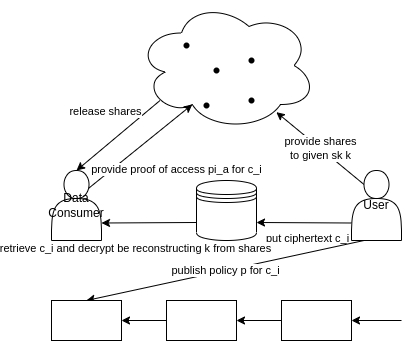
\includegraphics[width=0.4\textwidth]{figures/decentralized_access_control.png}
  \caption{Decentralized Access Control}
  \label{fig:decentralized_access_control}
\end{figure}
Fig. \ref{fig:decentralized_access_control} illustrates the steps required to share user data with a data consumer using the decentralized access control model.

For a given secret k, she computes a set of shares that gets sent to a committee of access controllers.

Using this secret k for a data item that is desirable to grant access to, the data item is encrypted and stored in the user's wallet or another storage system, and an access policy is published on-chain specifying under which conditions a data consumer is authorized to access the data item.

A data consumer wishing to access the data item is required to supply proof to the committee of access controller stating that the data consumer fulfills the access policy.

After validating the supplied proof from the data consumer the committee of access controllers releases the secret shares of the secret key k that was used for the encryption of the data item, the data consumer proved to have access to.

Using the shares and the ciphertext of the data item, the data consumer can successfully decipher it by reconstructing the secret k.

An Update to the access policy only requires the user to publish a new access policy to the distributed ledger.

\subsubsection{Additional Properties}
\begin{itemize}
  \item Data confidentiality
  \item Anonymity
  \item Auditability
  \item Policy Confidentiality
  \item Fair Access
  \item Access Revocation
\end{itemize}

\subsection{Decentralized Access Control with the Example of Calypso}

\section{Confidential yet Expressive Access Policies?}

\subsection{On-Chain Secrets}


\bibliographystyle{IEEEtran}
\bibliography{references}

\end{document}
